\documentclass[10pt,a4paper]{article}
\usepackage[latin1]{inputenc}
\usepackage{amsmath}
\usepackage{amsfonts}
\usepackage{amssymb}
\usepackage{graphicx}
\usepackage{longtable}
\usepackage{float}
\usepackage{physics}
\usepackage{soul}
\usepackage{caption}
\usepackage{subcaption}
\usepackage[section]{placeins}
\usepackage[left=2cm,right=2cm,top=2cm,bottom=2cm]{geometry}
\author{Akshat Mahajan}
\title{Physics 180Q - Two-Photon Interference}
\begin{document}
\maketitle
\noindent \textsl{This lab was performed in conjunction with Hanwen Qin.}
\section*{The Goal}
The purpose of this lab experiment was to demonstrate Hong-Ou-Mandel interference with down-converted photons. In particular, we measured the so-called \textit{coincidence dip} for a pair of photons impinging on detectors following transmission through a beam splitter. This refers to the minimum in coincidence count rates as the relative delay between single-photon wave packets approaches zero.
\section*{Theory}
This section indulges in a qualitative explanation of Hong-Ou-Mandel intereference. \\
\\
The interference effect can be summarised as so: when two indistinguishable particles emerge from a beam splitter with no path difference between them, the coincidence counts drop to zero. Conversely, if there \textit{is} a sizable path difference between them, coincidence counts rise to a non-zero level. In one sentence: \textit{indistinguishable particles destructively interfere with each other in a beam splitter.} For distinguishable particles, this effect does not come into play. For a broad spectrum of wavelengths for each particle, then, the coincidence counts do not drop completely to zero but do noticeably drop by some amount.
\section*{Measuring Two-Photon Interference}
We employed a blue laser source of 405 nm, which, when aimed at a BBO crystal, produces red laser light of 810 nm at an efficiency of about $10^{-11}$. These light beams were allowed to pass through a polarised 50:50 fiber optic coupling doubling as a linear beam splitter through to a mounted stage, where they were made to coincide on two detectors. A translation stage attached to one of the exit ports of the beam splitter enabled fine precision (upto 500 microns per twist of the handle) control over the path difference. By moving the translation stage, it was possible to change the path difference between the two exiting beams of light.
\begin{figure}[H]
\centering
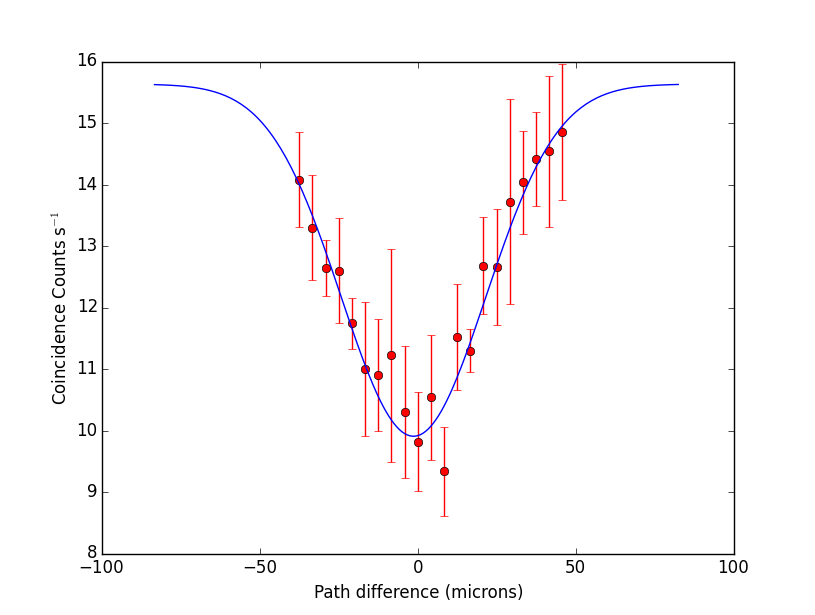
\includegraphics[scale=0.46]{../Analysis/figure_1.png}
\caption{Coincidence counts versus path difference with filters on. Red bars indicate standard error. The blue line indicates fit with Eq. (1) (see next page)}
\end{figure}
\noindent We originally went ahead and attached polarising filters to the detectors as well as the blue laser pump, ensuring that the vast majority of impinging light consisted of red 810 nm-centered wavepackets. Care was taken to try and keep all photons vertically aligned in polarisation - this ensures that there's a good overlap of spatial modes in the polarised fiber optic coupling, and thus a significant number of photons in the output. We first identified a minimum, then proceeded to carefully increment by 5 degrees in both directions until we were satisfied we had scanned the full range. Conversions to path difference were obtained from the fact that 60$^{\circ}$ resulted in a 50 $\mu$m displacement. The results can be seen in Fig. (1).\\
\\
Our distribution of coincidence counts was fit to the equation:
\begin{equation}
\mathrm{Counts} = C\cdot\left(T + R \right)\cdot\left(1 - 2\dfrac{\sqrt{TR}}{T+R}\exp{\dfrac{-\Delta k^{2} \Delta L^{2}}{2}}\right)
\end{equation}
where $C,T,R,$ and $\Delta k$ are all fits to the parameters. $T$ and $R$ are respectively analogues to the transmission and reflection coefficients, and their sum should appropriately be as close to 1 as possible. $\Delta k$ is a measure of the spread of the wavepacket that has been fed into the beam splitter.\\
\\
It is important to note that the degrees of freedom of the fit do not provide a unique fit to the data. Several nonlinear regression attempts with different initial conditions result in different solutions, all of them visually identical but with different $T,R,C$ and $\Delta k$. In order to arrive at the best fit, the heuristic $T + R = 1$ was applied - the fit shown in Fig. (1) satisfies that condition best out of ten different possible values, with realistic values of transmission and reflectivity. It may be noted that the full width half maximum of the resulting fit is about 50 $\mu$m - in line with what we'd expect.
\begin{table}[H]
\centering
\begin{tabular}{|c|c|c|c|}
\hline
$\Delta K$ & $C$ & $T$ & $R$\\
0.04 & 16.40 s$^{-1}$ & 0.919 & 0.033\\
\hline
\end{tabular}
\caption{Values of Fit Parameters for Fig. (1)}
\end{table}
We then proceeded to remove all of the filters, and therefore obtain much less pronounced interference. What we expect is that the FWHM of the resulting fit should be much narrower, since there is now greater spread in the wavepackets of the photon striking the detectors. As a rough figure, one would expect the $\Delta k$ to be about 10 $\mu$m. In practice, however, we did not obtain this result.
\begin{figure}[H]
\centering
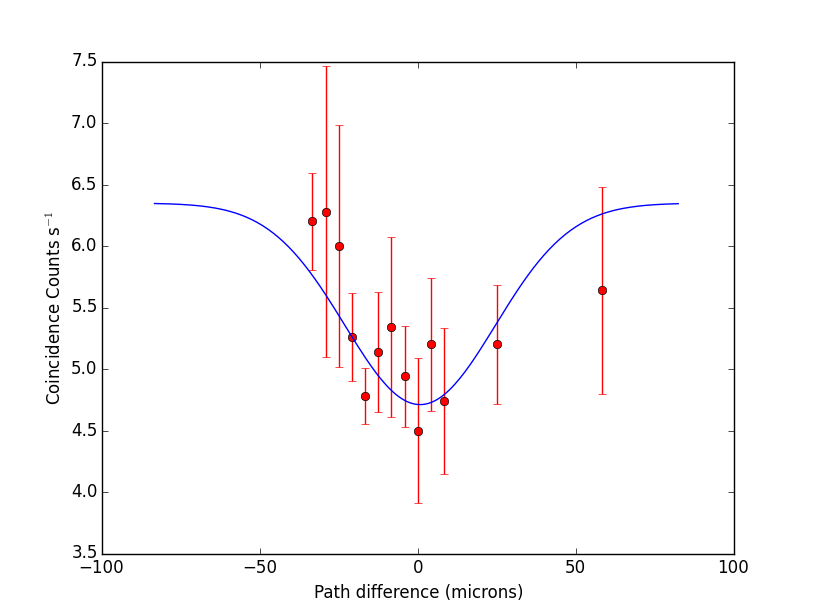
\includegraphics[scale=0.5]{../Analysis/figure_2.png}
\caption{Coincidence counts versus path difference with filters off. Red bars indicate standard error. The blue line indicates fit with Eq. (1)}
\end{figure}
\begin{table}[H]
\centering
\begin{tabular}{|c|c|c|c|}
\hline
$\Delta K$ & $C$ & $T$ & $R$\\
0.04 & 6.43 s$^{-1}$ & 0.969 & 0.016\\
\hline
\end{tabular}
\caption{Values of Fit Parameters for Fig. (2)}
\end{table}
\noindent Comparing Fig. (2) and Fig. (1), we notice two striking things:
\begin{itemize}
\item The photon coincidence counts are all much reduced with the filters off than the filters on.
\item The dip with the filters off is significantly shallower than the dip with the filters off, but both have the same spread in wavepackets.
\end{itemize}
It is not immediately obvious how to reconcile this behaviour with theory. We did note that the main thing that prompted this remarkable behaviour was the removal of the filter from the laser pump enclosure, while the behaviour was unaffected by the filters at the detectors. I advance the following hypothesis:
\begin{itemize}
\item By removing the filter, we may have inadvertently allowed horizontally aligned red particles to propagate through. This would result in a larger number of distinguishable particles, and thus a shallower dip.
\item Further, by removing the filters, we may have altered the number of photons being coupled through the fiber somehow.
\item Finally, by just removing the filters, we did \textit{not} alter the spread of the wavepackets. Blue light never enters our detectors - red laser light is still the only thing propagating through, with no added contributions from other waves\footnote{The lab lights were on during this time, and it has been argued in the past that they apparently have a red component in their spectrum - it can be argued that they do contribute to the red photons going through. However, this is perfectly alright - lab lights were on with and without filters, so we'd probably still get the same result anyway. The detectors may be tuned to only respond to the red spectrum of the light - a dubious hypothesis, but which can't be ruled out without further examination.}.
\end{itemize}
\end{document}